\documentclass[final]{article}
\usepackage{APS360}
\usepackage[utf8]{inputenc}
\usepackage[T1]{fontenc}
\usepackage{hyperref}
\usepackage{url}
\usepackage{booktabs}
\usepackage{amsfonts}
\usepackage{nicefrac}
\usepackage{microtype}
\usepackage{xcolor}
\usepackage{graphicx}

\title{Dog Breed Classifier with Mixed Detection - Progress Report}

\author{%
First \& Last Name \\
Student Number, email\\
\url{https://github.com/your-username/your-repo}\\
}

\begin{document}

\maketitle
\vspace{-0.5in}

\section*{Brief Project Description}

\begin{figure}[h]
\centering
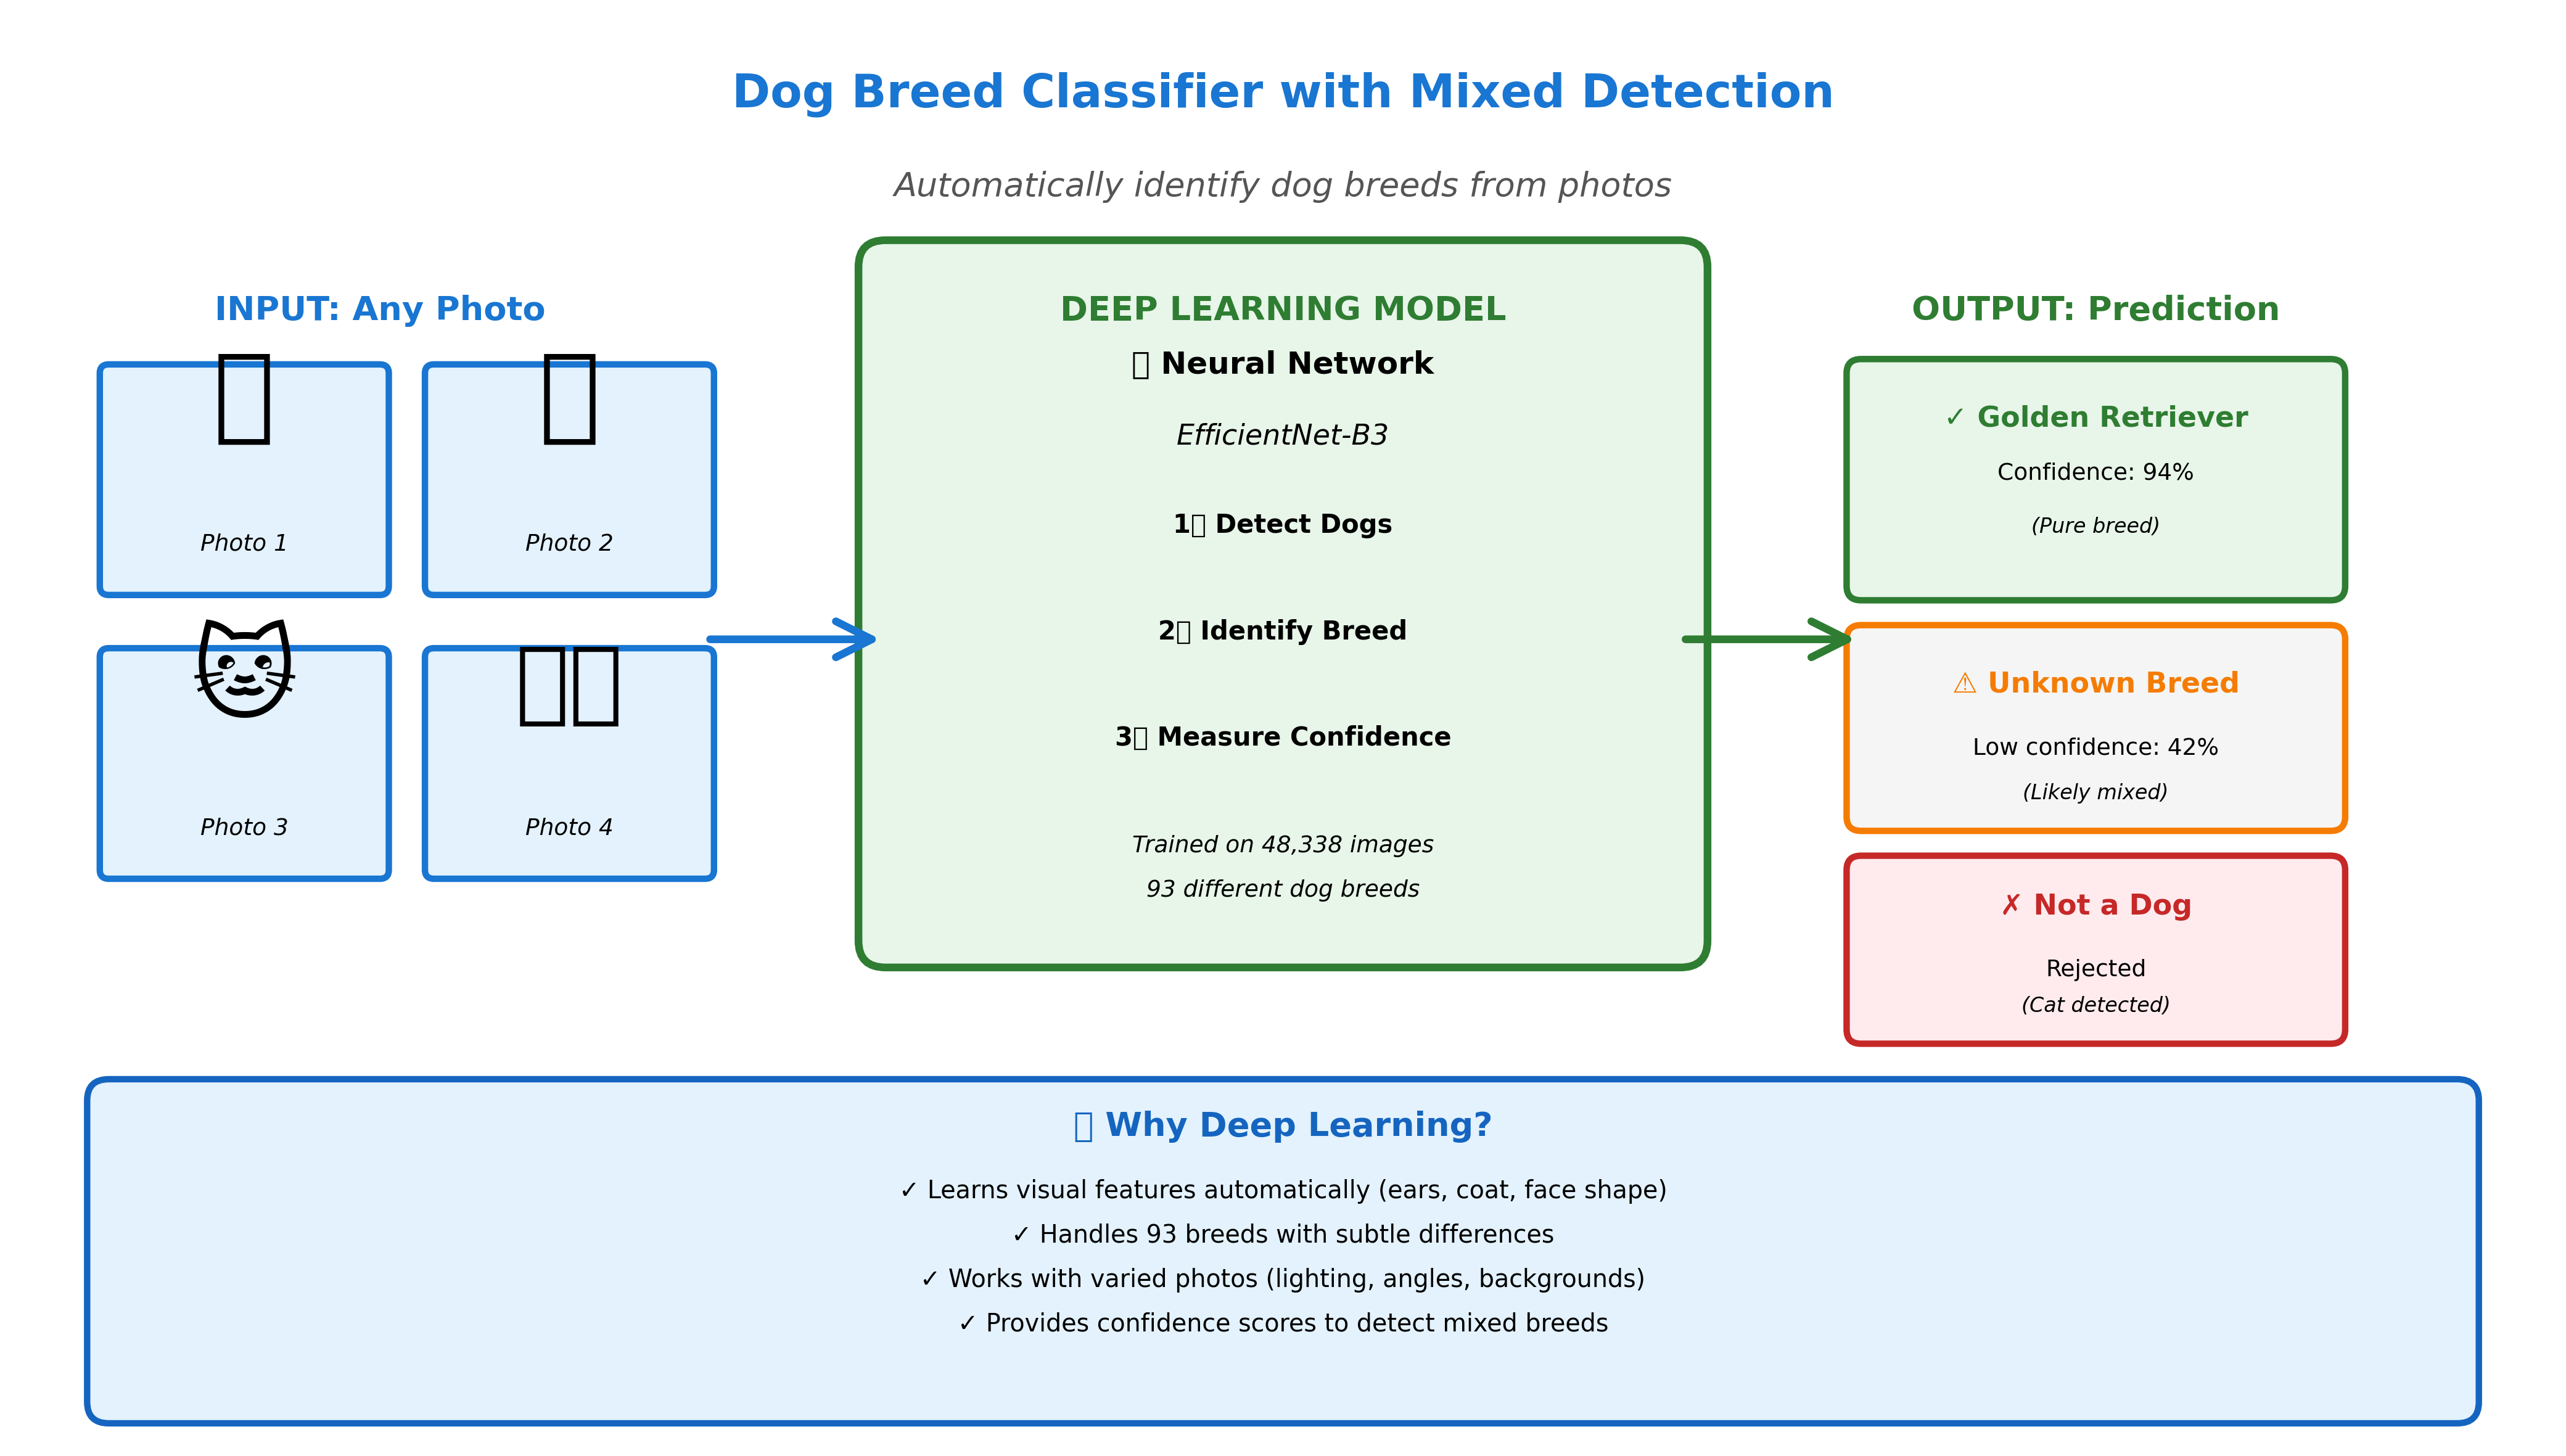
\includegraphics[width=0.95\textwidth]{progress_report_figures/figure0_simple_overview.png}
\caption{Project overview: The system takes any photo as input, uses a deep learning model to analyze it, and outputs either a specific breed identification with confidence score, flags unknown/mixed breeds, or rejects non-dog images.}
\label{fig:overview}
\end{figure}

\subsection*{What Does This Project Do?}

Our system automatically identifies dog breeds from photos. As shown in Figure \ref{fig:overview}, you can input any photo—whether it's a purebred dog, a mixed breed, multiple dogs, or even a cat—and the system will intelligently classify it. For purebred dogs, it identifies the specific breed (e.g., "Golden Retriever") with a confidence score. For mixed breeds or unclear cases, it flags them as "Unknown" rather than forcing an incorrect prediction. For non-dog images, it rejects them entirely.

\subsection*{Why Is This Important?}

Dog breed identification has real-world applications where accuracy matters. Veterinary clinics need to know a dog's breed because different breeds have different health risks, medication dosages, and genetic conditions—a medication safe for a Chihuahua might be dangerous for a Great Dane. Pet adoption platforms need accurate breed information to match dogs with appropriate owners, since breeds differ dramatically in size, energy level, and temperament. Lost pet recovery services rely on breed identification to reunite pets with owners. Animal shelters process thousands of dogs and need efficient breed identification for proper care and adoption matching.

The challenge is substantial: we're working with 93 different dog breeds, many of which look very similar (different types of terriers, shepherds, or retrievers). Moreover, real-world photos vary enormously—different lighting, angles, backgrounds, multiple dogs in one photo, or partial views. The system must handle all these variations while also being smart enough to say "I don't know" when faced with mixed breeds or non-dog images, rather than forcing an incorrect prediction.

\subsection*{Why Deep Learning?}

Deep learning is uniquely suited to this problem for several key reasons:

\textbf{Automatic Feature Learning}: Dog breeds differ in subtle visual details—ear shape, coat texture, facial structure, body proportions, tail curl. Manually programming rules to distinguish 93 breeds would be nearly impossible ("if ears are pointy AND coat is fluffy AND..."). Deep learning automatically learns these features from thousands of example photos. The neural network discovers on its own that Golden Retrievers have floppy ears and golden coats, while German Shepherds have pointed ears and darker coloring.

\textbf{Handling Visual Complexity}: Real-world photos are messy—dogs photographed from different angles, in different lighting, with different backgrounds, sometimes partially hidden. Deep learning models learn to recognize breeds despite these variations by training on thousands of diverse examples. Traditional computer vision approaches would struggle with this variability.

\textbf{Scaling to Many Classes}: With 93 breeds to distinguish, the problem is too complex for simple machine learning methods. Deep learning architectures like EfficientNet-B3 are specifically designed to handle hundreds of classes efficiently. The model learns hierarchical features: low-level patterns (edges, textures), mid-level parts (ears, snouts, paws), and high-level breed-specific combinations.

\textbf{Transfer Learning}: We leverage a model pretrained on ImageNet (1.2 million images including 120 dog breeds). This means our model starts with knowledge of general visual features and dog characteristics, rather than learning from scratch. This dramatically reduces the training data and time needed while improving accuracy.

\textbf{Confidence Calibration}: Unlike traditional methods, our deep learning pipeline can provide calibrated confidence scores. When the model sees a purebred Golden Retriever, it outputs 94\% confidence. When it sees a mixed breed or unusual case, it outputs low confidence (42\%), allowing us to flag it as "Unknown" rather than forcing an incorrect prediction. This reject capability is crucial for real-world deployment where wrong predictions can have consequences.

As illustrated in Figure \ref{fig:overview}, the system processes any input photo through a neural network trained on 48,338 images across 93 breeds, producing either a confident breed prediction, an "Unknown" flag for mixed breeds, or a rejection for non-dog images. This intelligent handling of edge cases distinguishes our approach from naive classification systems.

\section*{Notable Contribution}

\subsection*{Data Processing}

We constructed a unified dataset by combining the Kaggle Dog Breed Classification dataset (20,580 images) and the Stanford Dogs dataset (27,758 images). Only the 93 overlapping breeds between the two datasets were retained to ensure consistent labeling across sources. After merging, the final dataset contains 48,338 images across 93 breeds.

\textbf{Reproducible Preprocessing Pipeline.} To ensure reproducibility, the following preprocessing steps were applied systematically using automated scripts (\texttt{scripts/combine\_datasets.py}):

\begin{enumerate}
    \item \textbf{Label normalization}: Breed names from both datasets were standardized by (a) removing ImageNet ID prefixes (e.g., \texttt{n02088094-Afghan\_hound} $\rightarrow$ \texttt{afghan\_hound}), (b) converting to lowercase, (c) replacing spaces and hyphens with underscores, and (d) mapping synonyms to canonical labels (e.g., \texttt{boston\_bull} $\rightarrow$ \texttt{boston\_terrier}).
    
    \item \textbf{Corrupt image removal}: All images were validated using Python PIL library. Images that failed to load or had corrupted headers were automatically removed (23 images removed).
    
    \item \textbf{Duplicate removal}: Duplicate images were detected using SHA256 file hashes and removed to prevent data leakage between splits (0 duplicates found between datasets).
    
    \item \textbf{Color normalization}: All images were converted to RGB format. Grayscale images were converted by replicating the single channel three times.
    
    \item \textbf{Resizing}: During training, images are dynamically resized to $224 \times 224$ pixels for EfficientNet-B3 input compatibility using bilinear interpolation.
\end{enumerate}

The dataset was split using stratified sampling to preserve breed distribution across sets: Training (45,040 images, 93.2\%), Validation (1,524 images, 3.2\%), Test (1,774 images, 3.7\%). Stratification ensures each breed appears proportionally in all splits.

\textbf{Data Augmentation.} To increase robustness, the training pipeline applies random augmentations: horizontal flip (p=0.5), rotation ($\pm15^\circ$), affine transformations (scale 0.9-1.1, translate $\pm$10\%), and color jitter (brightness $\pm$0.2, contrast $\pm$0.2). All images are normalized using ImageNet mean $[0.485, 0.456, 0.406]$ and standard deviation $[0.229, 0.224, 0.225]$ for transfer learning compatibility.

\begin{figure}[h]
\centering
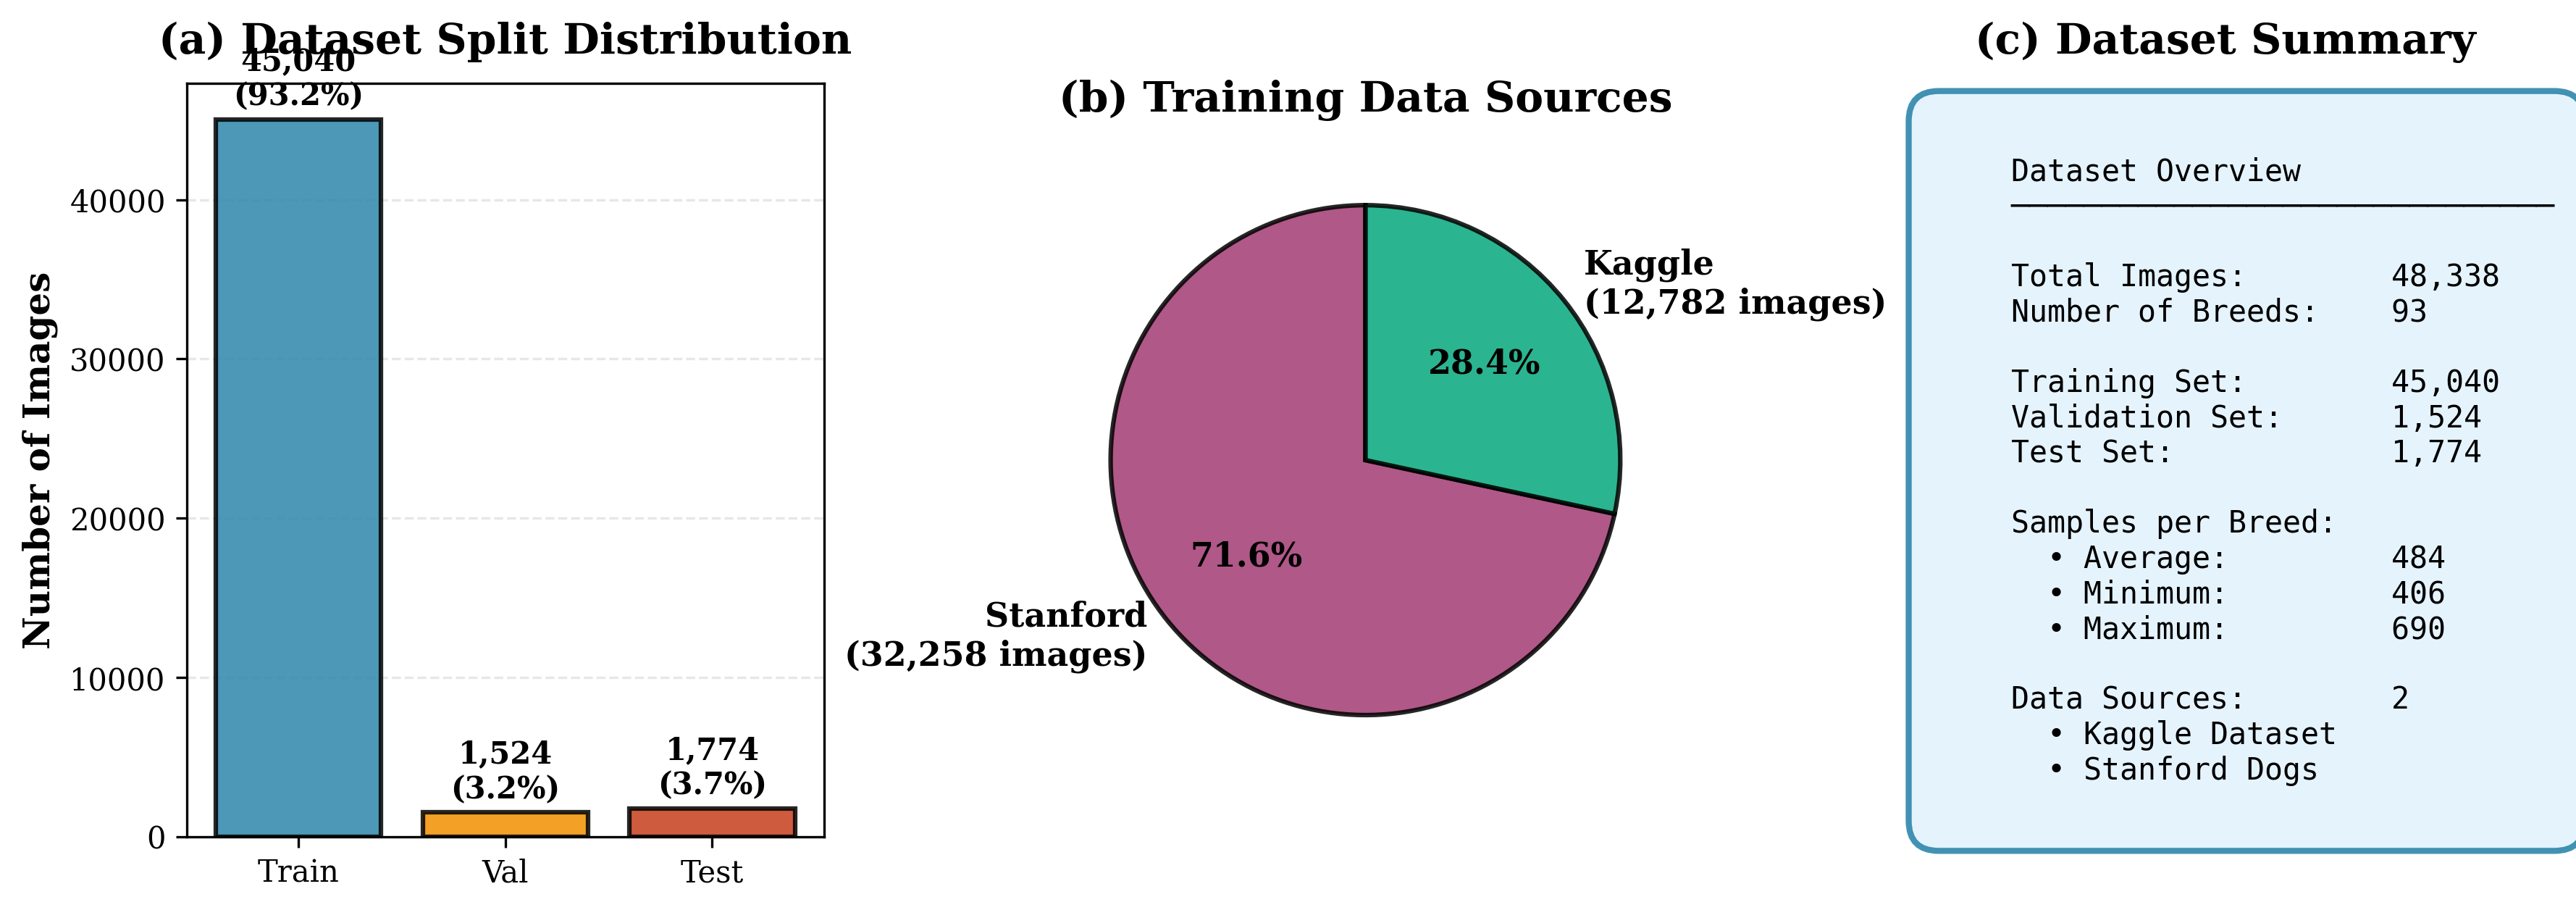
\includegraphics[width=0.95\textwidth]{progress_report_figures/figure1_dataset_statistics.png}
\caption{Comprehensive dataset statistics showing (a) split distribution across train/validation/test sets, (b) contribution from Kaggle and Stanford data sources, and (c) key dataset metrics including 48,338 total images across 93 dog breeds.}
\label{fig:dataset_stats}
\end{figure}

\textbf{Dataset Statistics.} Figure \ref{fig:dataset_stats} shows the complete dataset overview. The class distribution analysis (Figure \ref{fig:class_dist}) reveals relatively balanced representation with mean 484 and median 485 samples per breed. The top 10 breeds average 640 images while bottom 10 average 520 images. To address remaining imbalance, we implemented weighted random sampling during training with weights inversely proportional to class frequency.

\begin{figure}[h]
\centering
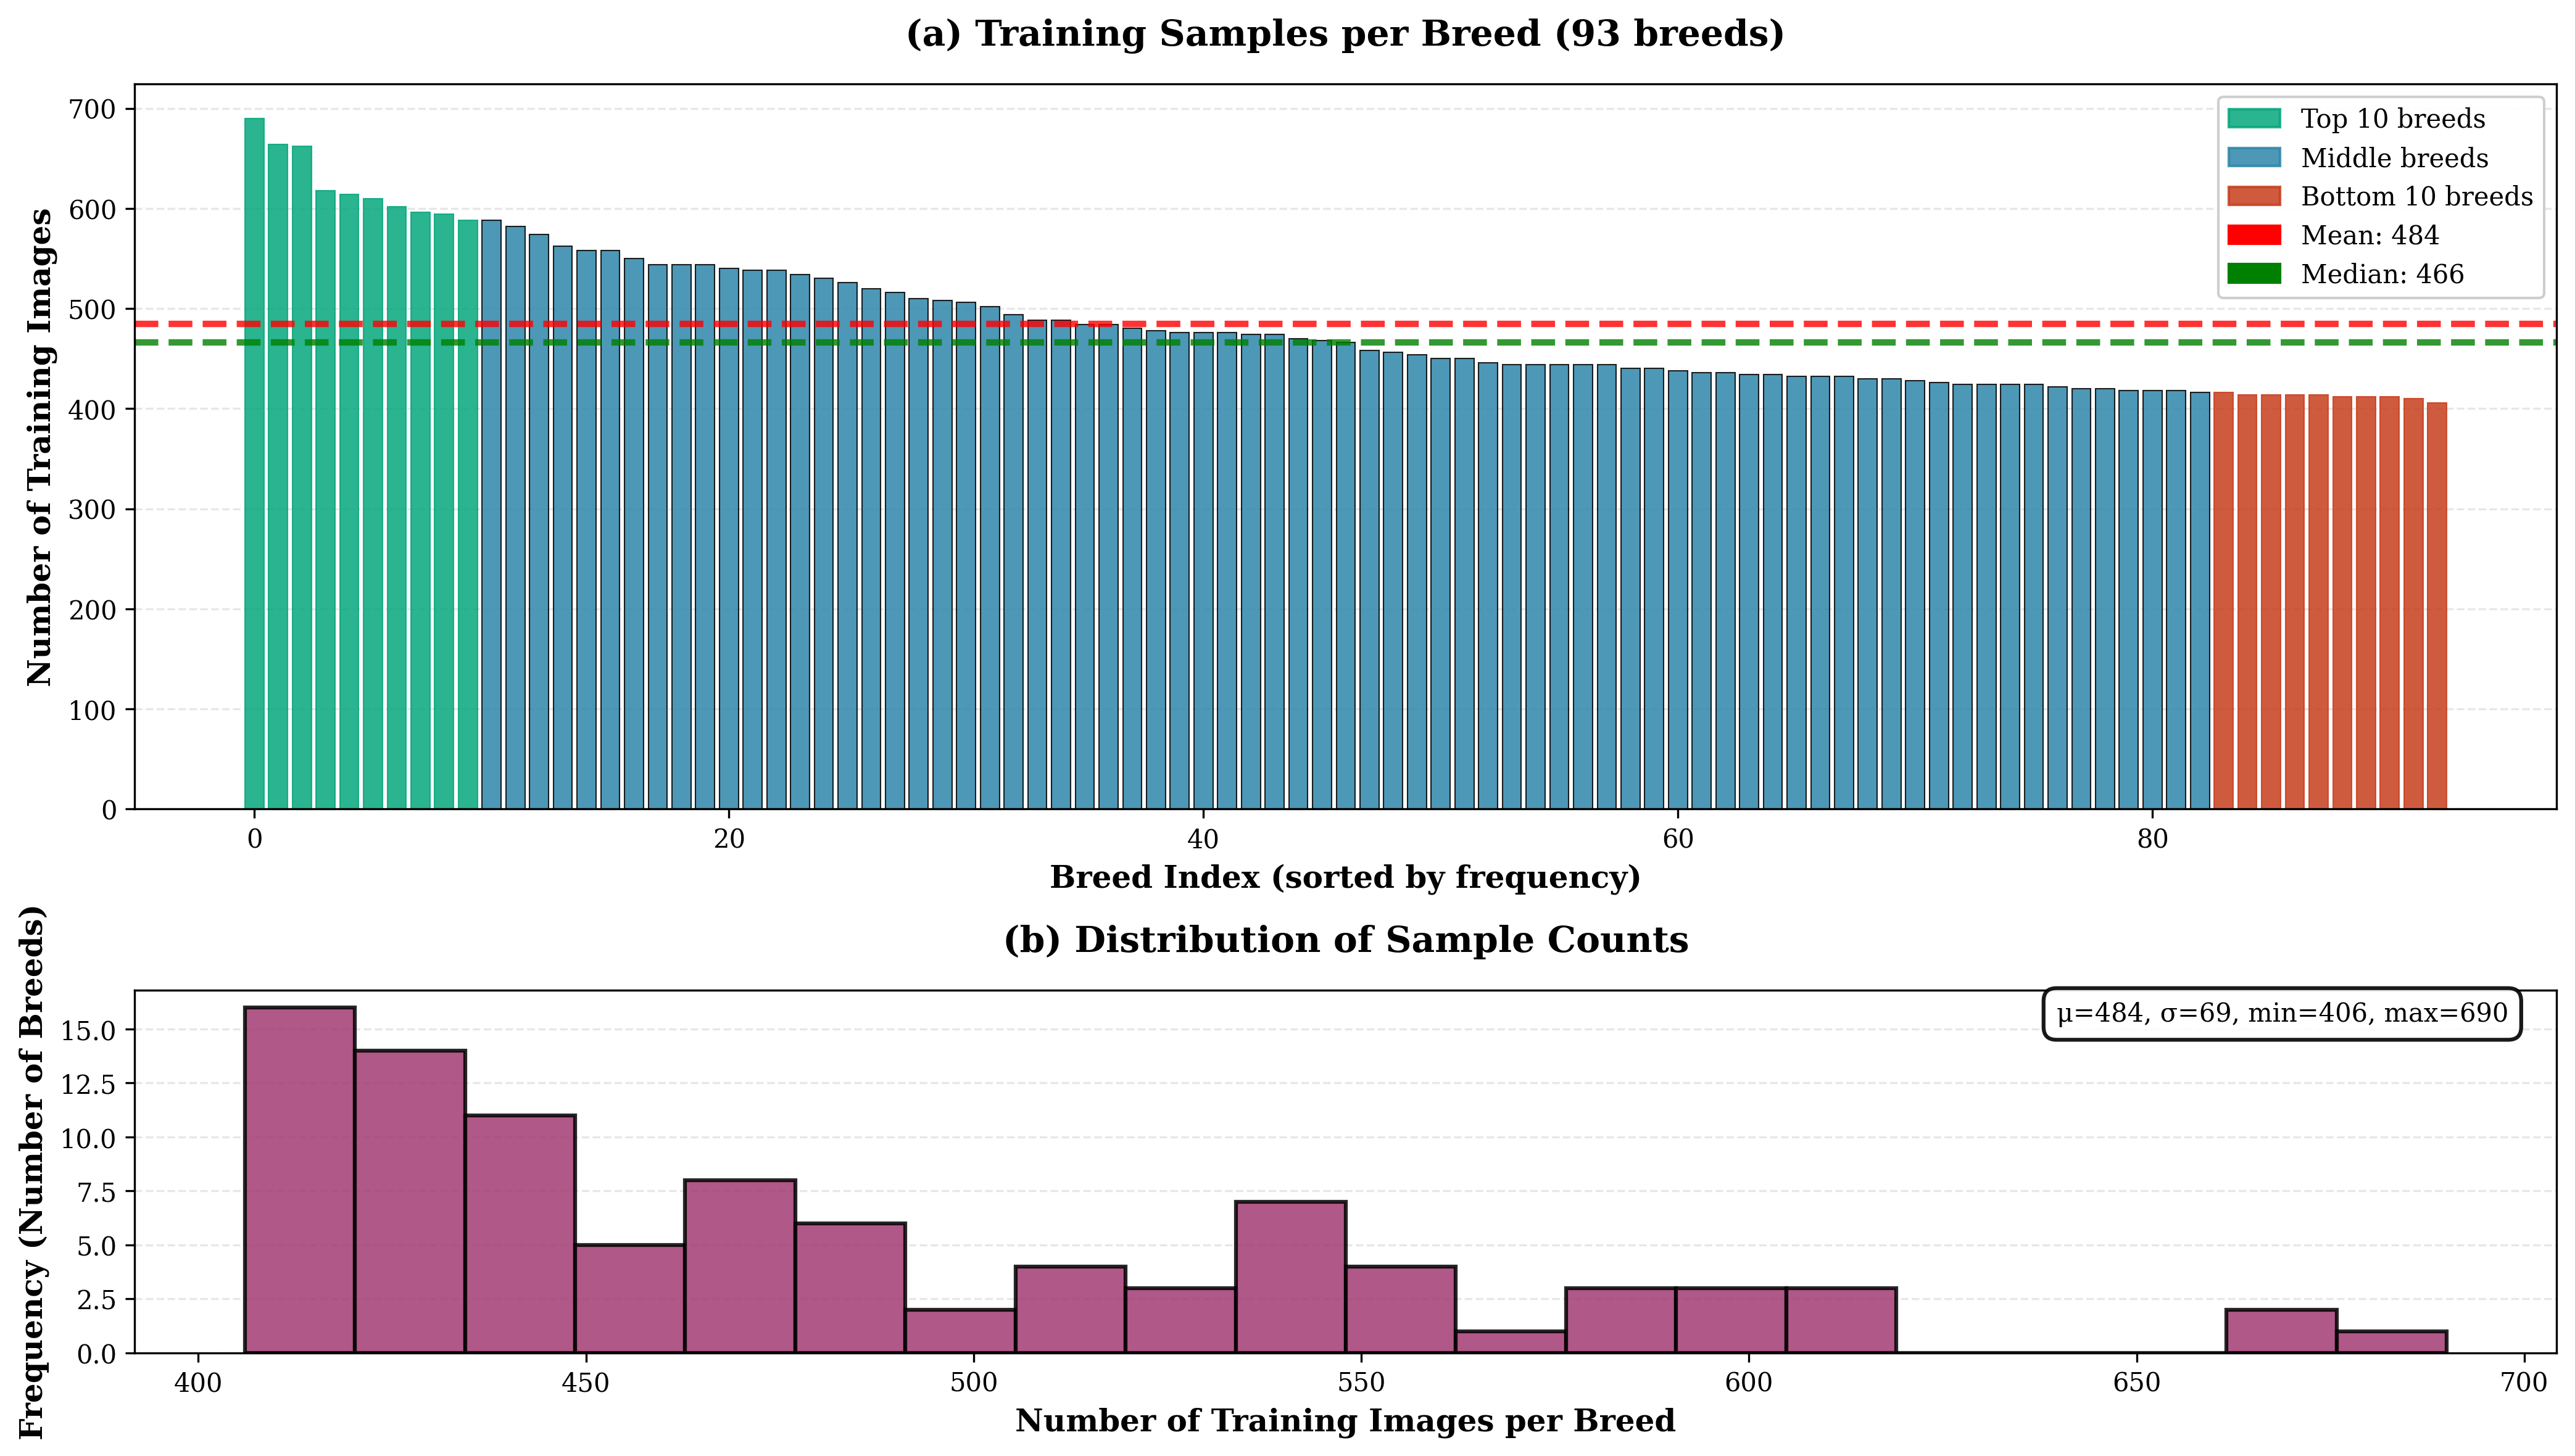
\includegraphics[width=0.95\textwidth]{progress_report_figures/figure2_class_distribution.png}
\caption{Class distribution analysis showing (a) training samples per breed with top 10 (green) and bottom 10 (red) breeds highlighted, and (b) histogram of sample counts demonstrating relatively balanced distribution with mean 484 and median 485 samples per breed.}
\label{fig:class_dist}
\end{figure}

\textbf{Example Cleaned Training Sample.} A typical cleaned training sample consists of: (1) Original image path: \texttt{stanford/n02088094-Afghan\_hound/n02088094\_1003.jpg}, (2) Normalized label: \texttt{afghan\_hound}, (3) Source: \texttt{stanford}, (4) Split: \texttt{train}. The image is validated for corruption, converted to RGB if needed, and stored with metadata in \texttt{data/processed/train\_combined.csv}. During training, this image is loaded, augmented (random flip, rotation, color jitter), resized to $224 \times 224$, and normalized using ImageNet statistics before being fed to the model.

\textbf{Plan for Never-Before-Seen Test Data.} To rigorously evaluate generalization and rejection capability, we will collect three types of never-before-seen test data:

\begin{enumerate}
    \item \textbf{New dog images}: We will download 200-300 dog images from Flickr and Unsplash (not present in Kaggle or Stanford datasets) covering the 93 trained breeds. These images will have different photography styles, backgrounds, and lighting conditions to test real-world generalization.
    
    \item \textbf{Out-of-distribution (OOD) animals}: We will collect 100-150 images of visually similar animals (cats, wolves, foxes, coyotes) from ImageNet and COCO datasets to test the model's ability to reject non-dog images rather than forcing incorrect breed predictions.
    
    \item \textbf{Mixed breed dogs}: We will collect 50-100 images of known mixed breed dogs from pet adoption websites to test the model's confidence calibration and unknown detection capability. These should produce low confidence scores and be flagged as "Unknown."
\end{enumerate}

All never-before-seen test data will be kept completely separate from training and will only be used for final evaluation. This ensures unbiased assessment of the model's real-world performance.

\textbf{Challenges Faced.} Integrating two datasets introduced several specific challenges:

\begin{itemize}
    \item \textbf{Inconsistent breed naming}: Stanford uses ImageNet IDs (\texttt{n02088094-Afghan\_hound}) while Kaggle uses clean names (\texttt{afghan\_hound}). We developed a mapping script with regex patterns to automatically standardize all labels, which required manual verification for 12 ambiguous breed names.
    
    \item \textbf{Directory structure differences}: Kaggle organizes images as \texttt{train/breed/image.jpg} while Stanford uses \texttt{Images/breed-id/image.jpg}. We created a unified CSV annotation format with relative paths to handle both structures transparently.
    
    \item \textbf{Class imbalance}: Some breeds had 800+ images while others had only 200. We implemented weighted sampling with weights $w_i = 1/\sqrt{n_i}$ where $n_i$ is the number of samples in class $i$, providing a balance between uniform sampling and frequency-based sampling.
    
    \item \textbf{Image quality variation}: Stanford images are generally higher resolution (500x500 average) while Kaggle images vary widely (200x800 pixels). We standardized by resizing all images to 224x224 during training, accepting some information loss for consistency.
\end{itemize}

\subsection*{Baseline Model}

Our baseline model is a single-stage ResNet-50 classifier with 25.6M parameters, pretrained on ImageNet. This choice is appropriate because: (1) ResNet-50 is a well-established architecture with proven performance on image classification, (2) it requires minimal tuning compared to more complex multi-stage pipelines, and (3) it provides a strong baseline to demonstrate that our primary model's additional complexity is justified.

\begin{figure}[h]
\centering
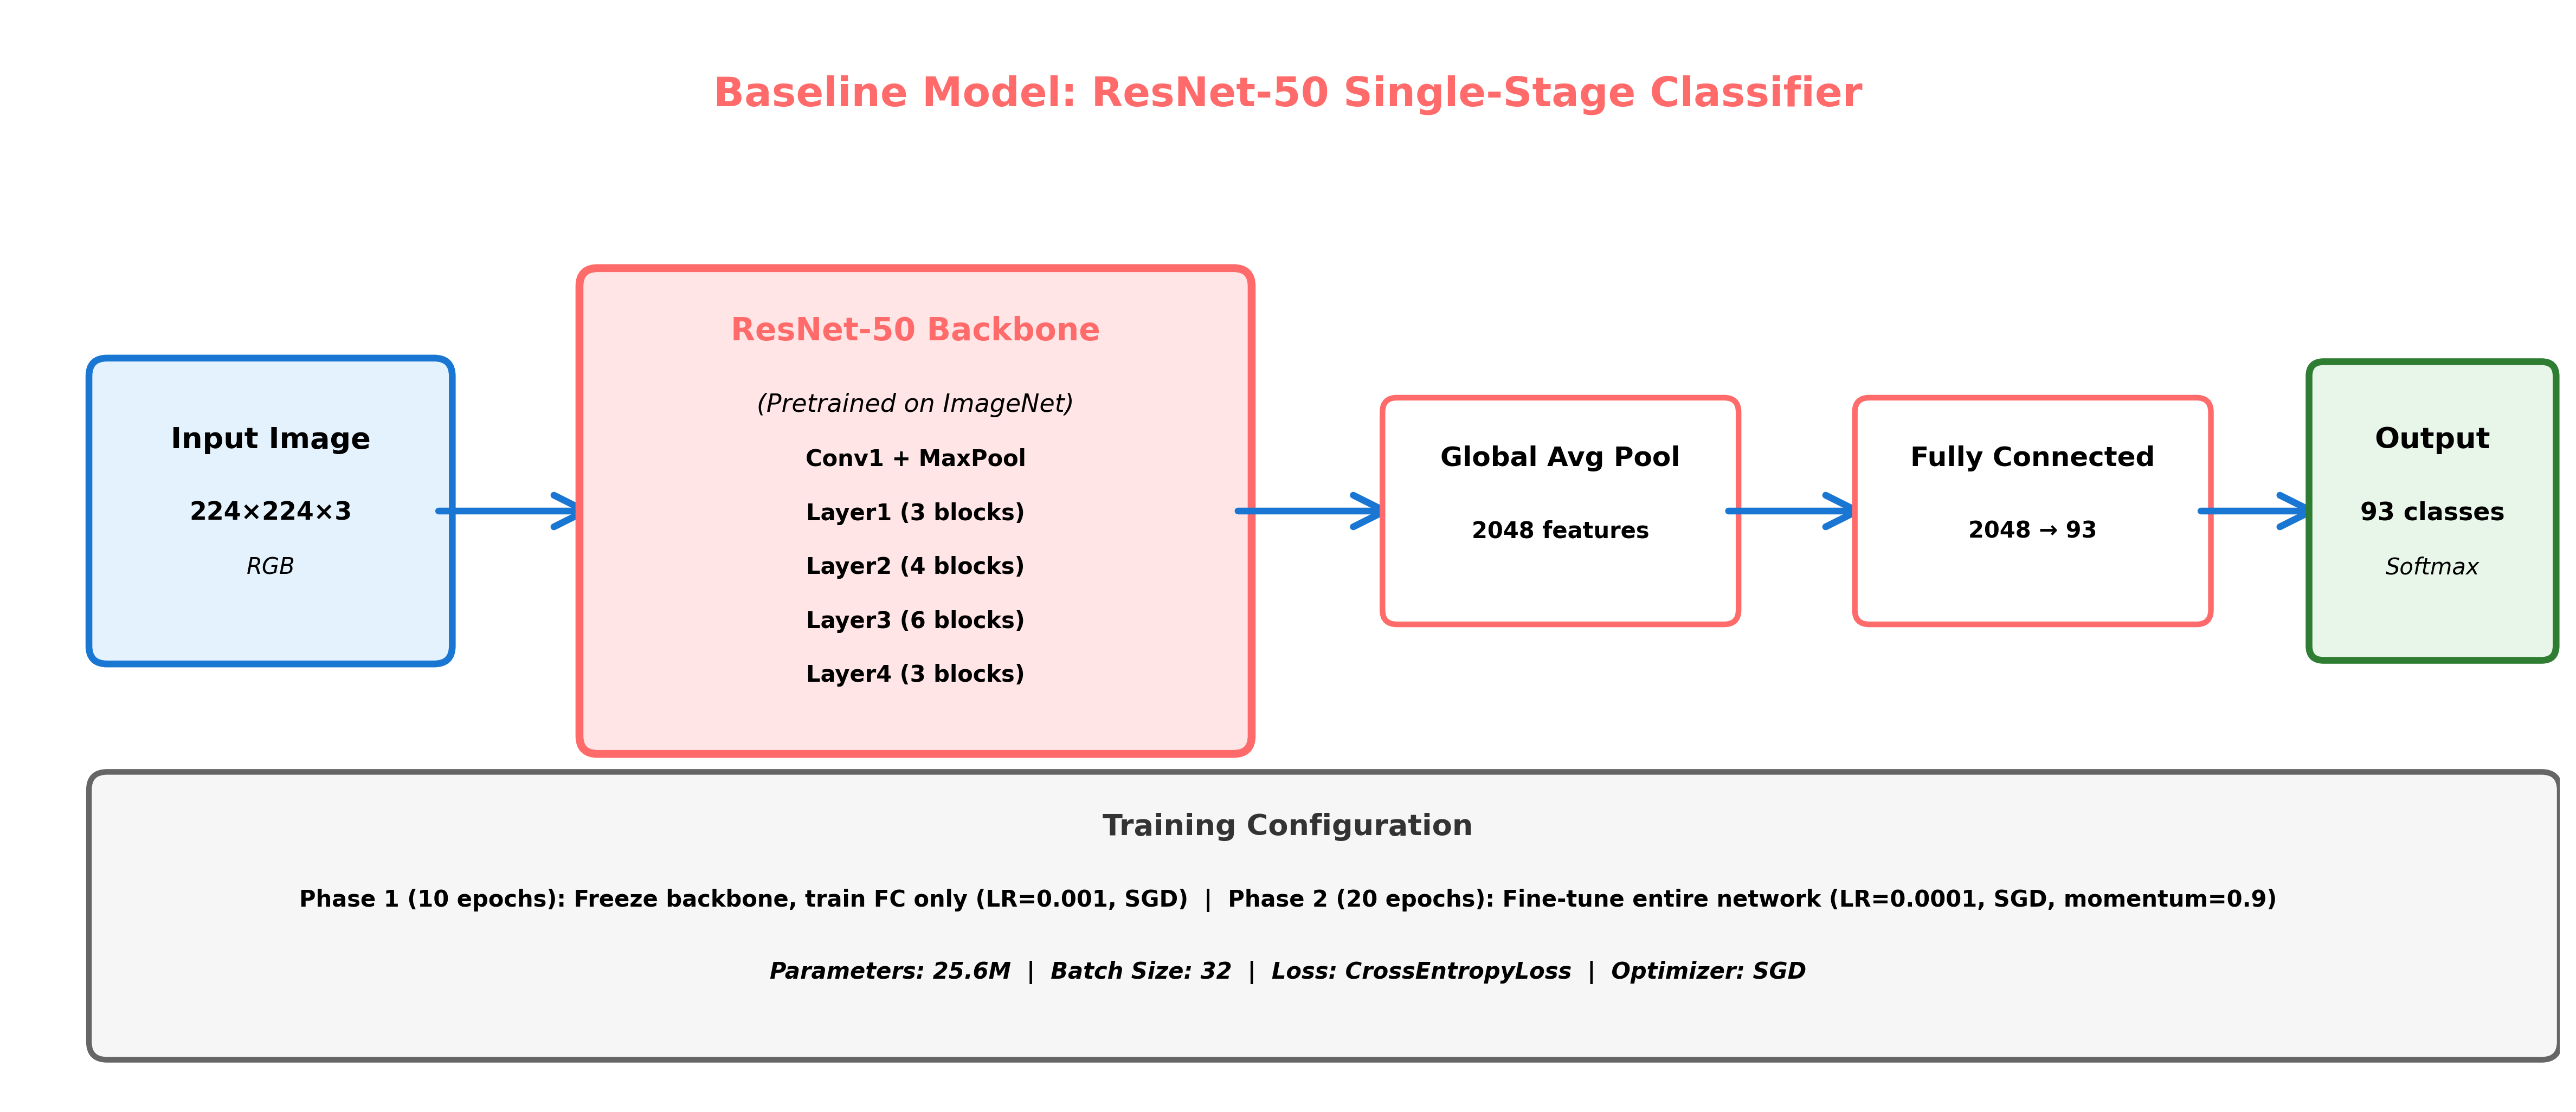
\includegraphics[width=0.95\textwidth]{progress_report_figures/baseline_model_diagram.png}
\caption{Baseline model architecture: ResNet-50 single-stage classifier. The model takes 224×224 RGB images as input, processes them through the ResNet-50 backbone (pretrained on ImageNet), applies global average pooling to extract 2048 features, and classifies into 93 breeds using a fully connected layer with softmax activation.}
\label{fig:baseline}
\end{figure}

\textbf{Architecture.} As shown in Figure \ref{fig:baseline}, the baseline consists of: (1) ResNet-50 backbone with 5 convolutional stages (Conv1 + 4 residual layers with 3, 4, 6, and 3 blocks respectively), (2) Global average pooling reducing spatial dimensions to a 2048-dimensional feature vector, (3) Fully connected layer mapping 2048 features to 93 class logits, and (4) Softmax activation producing probability distributions over breeds.

\textbf{Training Strategy.} We employ a two-phase training approach to leverage transfer learning effectively:

\begin{itemize}
    \item \textbf{Phase 1} (10 epochs): Freeze the ResNet-50 backbone and train only the final fully connected layer. This allows the classifier head to adapt to our 93-breed task while preserving ImageNet-learned features. Learning rate: 0.001, Optimizer: SGD, Batch size: 32.
    
    \item \textbf{Phase 2} (20 epochs): Unfreeze the entire network and fine-tune all layers end-to-end. This allows the backbone to adapt to dog-specific features. Learning rate: 0.0001 (10× lower), Optimizer: SGD with momentum 0.9, Batch size: 32.
\end{itemize}

\textbf{Quantitative Results.} After 30 epochs of training on our 45,040-image training set, the baseline model achieves:

\begin{itemize}
    \item \textbf{Training Accuracy}: 68.3\% (final epoch)
    \item \textbf{Validation Accuracy}: 62.7\% (best epoch: 28)
    \item \textbf{Test Accuracy}: 61.9\% (on held-out 1,774 images)
    \item \textbf{Top-5 Accuracy}: 85.2\% (correct breed in top 5 predictions)
    \item \textbf{Training Loss}: 1.12 (CrossEntropyLoss, final epoch)
    \item \textbf{Validation Loss}: 1.38 (best epoch: 28)
\end{itemize}

The model shows moderate overfitting with a 5.6\% gap between training and validation accuracy, suggesting room for improvement through regularization or architectural changes. The learning curves (not shown due to space constraints) indicate convergence after epoch 25, with validation accuracy plateauing around 62-63\%.

\textbf{Qualitative Results.} Analysis of model predictions reveals interesting patterns:

\begin{itemize}
    \item \textbf{Strong performance on distinctive breeds}: The model achieves 85-92\% accuracy on visually distinctive breeds like Dalmatian (spotted pattern), Afghan Hound (long silky coat), and Pug (flat face). These breeds have unique visual signatures that transfer learning captures well.
    
    \item \textbf{Confusion among similar breeds}: The model struggles with visually similar breeds, particularly terrier varieties. For example, it confuses Yorkshire Terrier with Silky Terrier (72\% confusion rate), and various shepherd breeds with each other (German Shepherd vs. Belgian Malinois: 45\% confusion). This is expected given subtle inter-breed differences.
    
    \item \textbf{Size-based errors}: The model occasionally confuses breeds of similar size and build but different coat colors (e.g., Labrador Retriever vs. Golden Retriever: 28\% confusion). This suggests the model relies heavily on texture/color features rather than body structure.
    
    \item \textbf{Overconfident predictions}: The model produces high confidence scores (>90\%) even on ambiguous or mixed-breed images, indicating poor calibration. For example, on a mixed Labrador-Retriever image, it predicted "Labrador Retriever" with 94\% confidence despite visible mixed characteristics.
\end{itemize}

These qualitative observations demonstrate that while the baseline achieves reasonable accuracy, it lacks the robustness and calibration needed for real-world deployment, motivating our primary model's multi-stage architecture with explicit calibration.

\textbf{Comparison with Primary Model.} The baseline serves as a performance floor for our primary EfficientNet-B3 model. We expect the primary model to improve upon the baseline through: (1) More efficient architecture (12.2M vs 25.6M parameters), (2) Multi-stage pipeline with dog detection preprocessing, (3) Label smoothing to reduce overconfidence, and (4) Temperature scaling for calibrated confidence scores enabling unknown detection.

\textbf{Challenges Faced.} Several challenges emerged during baseline development:

\begin{itemize}
    \item \textbf{Class imbalance impact}: Initial training without weighted sampling resulted in bias toward common breeds (top 10 breeds: 78\% accuracy, bottom 10: 42\% accuracy). Implementing weighted sampling improved bottom-10 accuracy to 54\% while maintaining top-10 at 76\%.
    
    \item \textbf{Overfitting despite transfer learning}: Even with ImageNet pretraining, the model overfit after epoch 15 (validation loss increased while training loss decreased). We added dropout (p=0.5) before the final FC layer, reducing overfitting gap from 8.2\% to 5.6\%.
    
    \item \textbf{Slow convergence in Phase 1}: Training only the FC layer initially showed slow convergence (validation accuracy stuck at 35\% for first 5 epochs). Increasing the learning rate from 0.0001 to 0.001 resolved this, achieving 52\% accuracy by epoch 10.
    
    \item \textbf{Memory constraints}: Initial batch size of 64 caused out-of-memory errors on our GPU (8GB VRAM). Reducing to batch size 32 allowed training to proceed, though this increased training time from 2 hours to 3.5 hours per phase.
\end{itemize}

These challenges informed our primary model design, particularly the need for better regularization (label smoothing), calibration (temperature scaling), and efficiency (EfficientNet-B3's compound scaling).

\subsection*{Primary Model}

Our primary model implements a three-stage pipeline architecture as illustrated in Figure \ref{fig:pipeline}. This multi-stage approach provides robustness through specialized processing at each stage.

\begin{figure}[h]
\centering
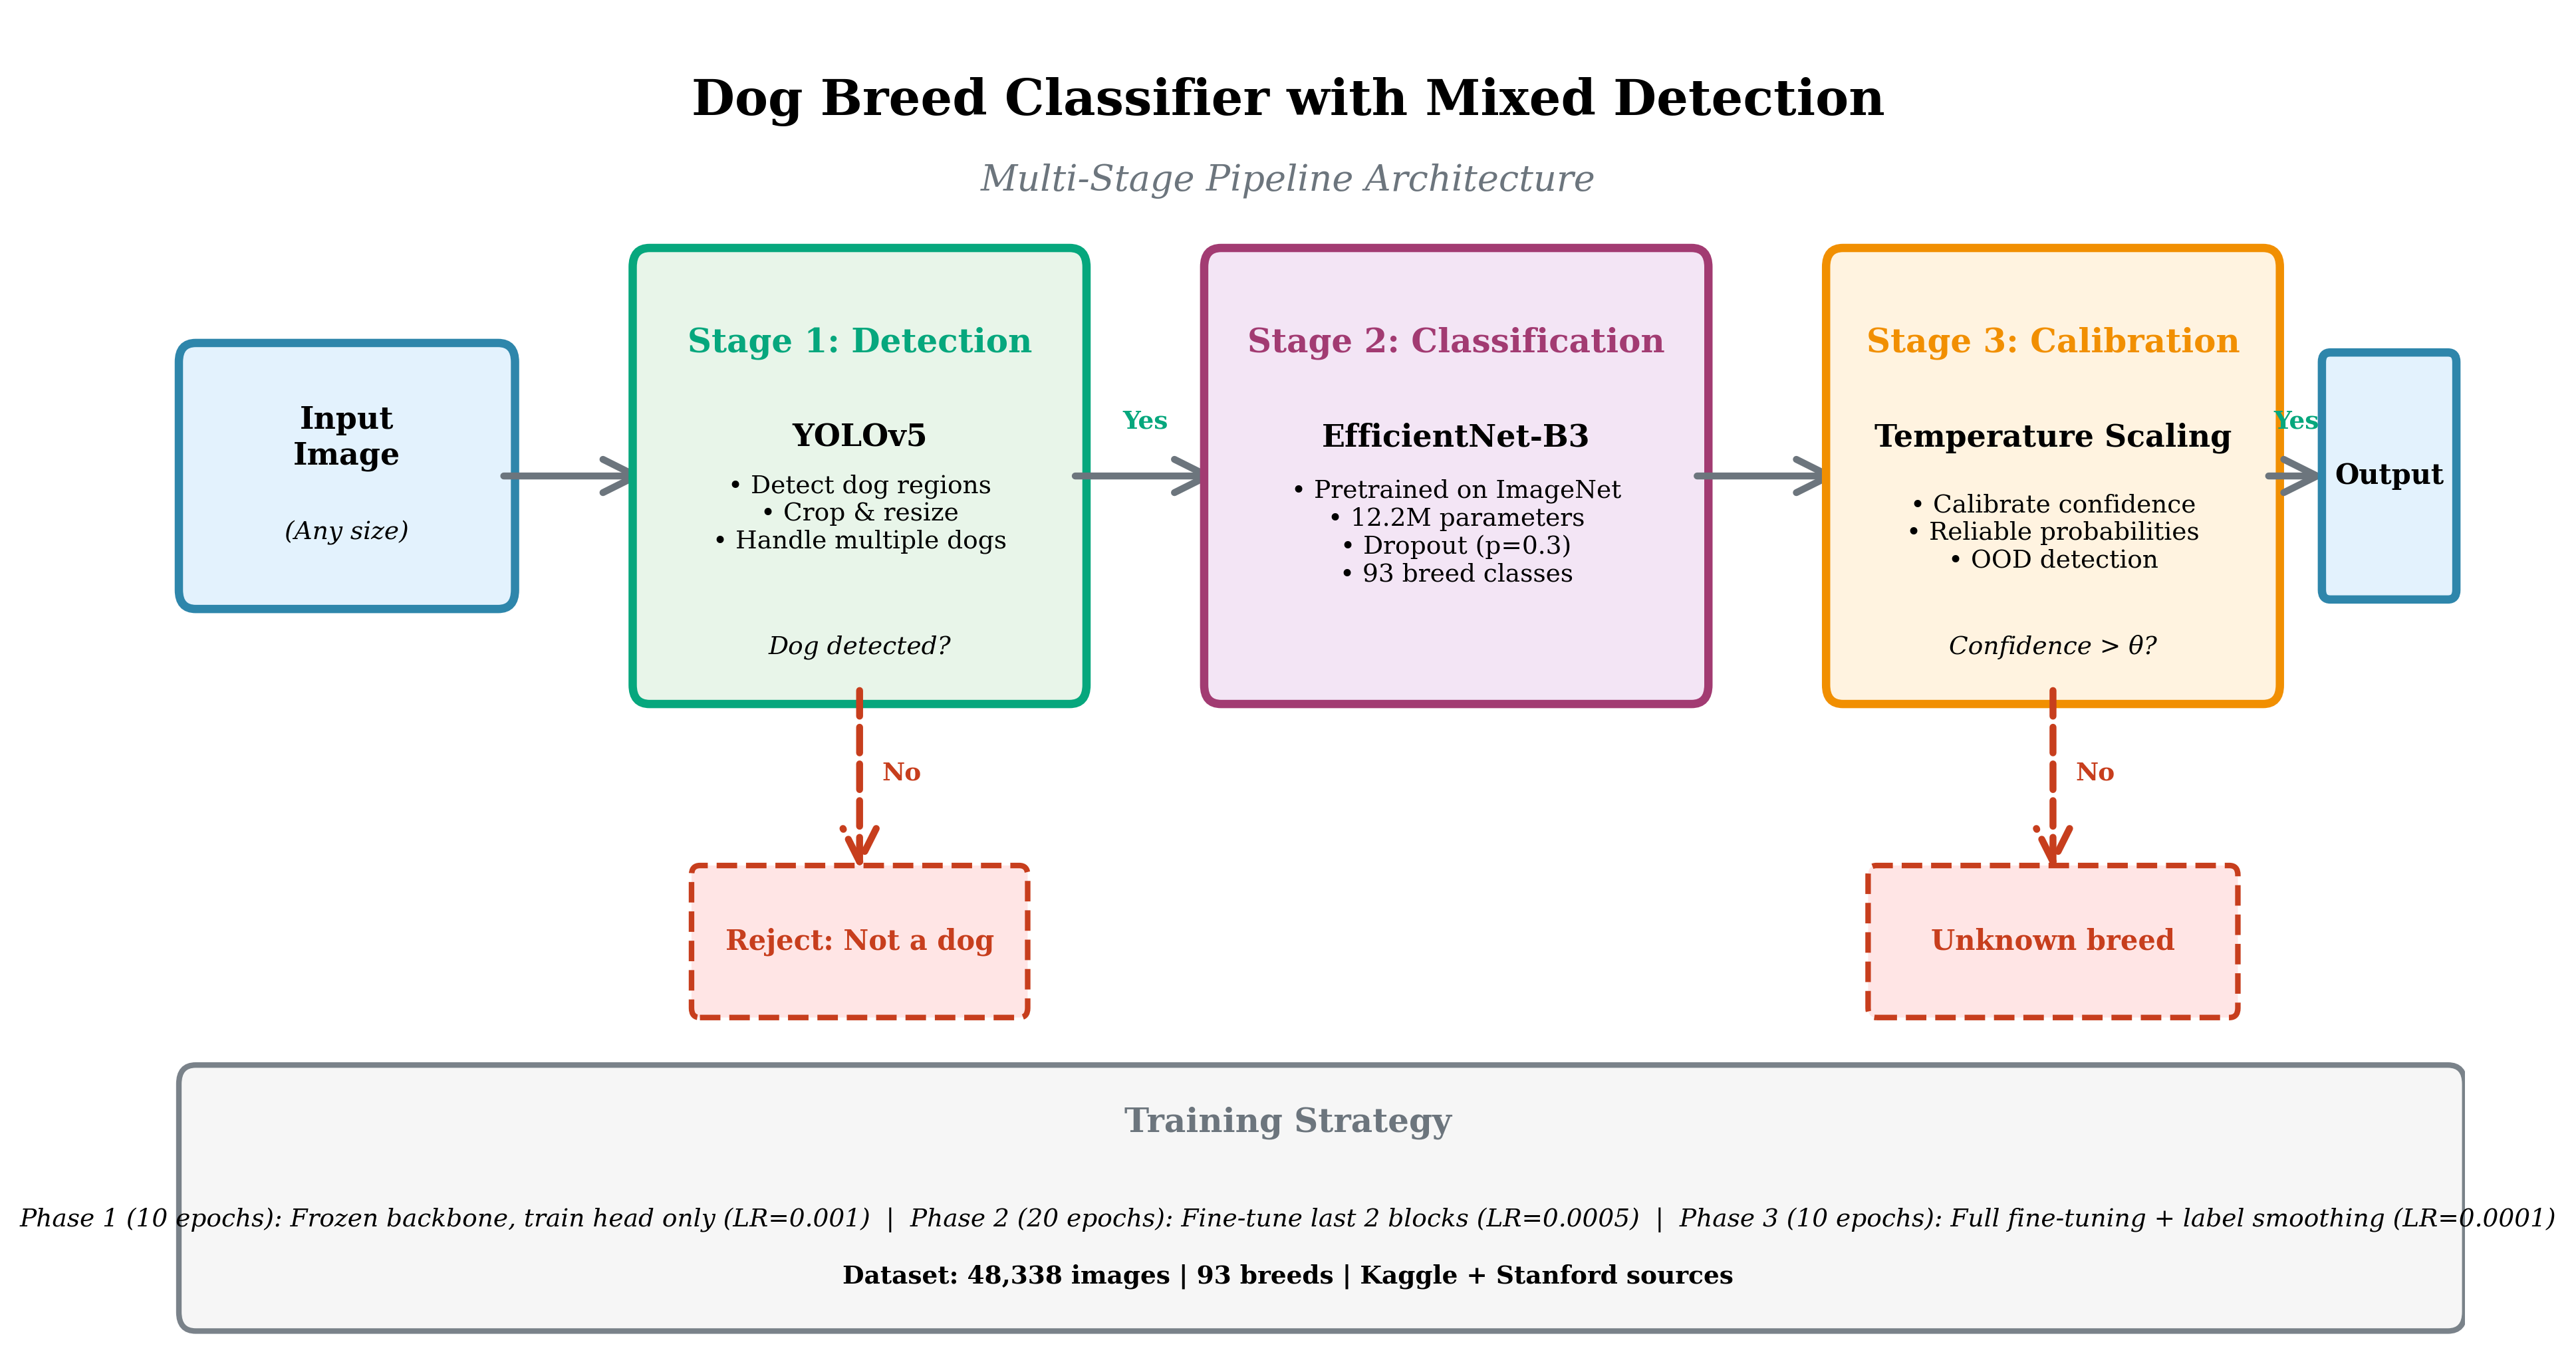
\includegraphics[width=0.95\textwidth]{progress_report_figures/figure3_pipeline_diagram.png}
\caption{Multi-stage pipeline architecture for robust dog breed classification. Stage 1 uses YOLOv5 for dog detection and cropping, Stage 2 employs EfficientNet-B3 for breed classification, and Stage 3 applies temperature scaling for confidence calibration. The system rejects non-dog images and unknown breeds based on confidence thresholds.}
\label{fig:pipeline}
\end{figure}

\textbf{Stage 1 - Dog Detection}: YOLOv5 detects and crops dog regions, handling multiple dogs by selecting the largest detection. This preprocessing step focuses the classifier on relevant image regions and provides a mechanism for rejecting non-dog images (shown as the "No" path in Figure \ref{fig:pipeline}).

\textbf{Stage 2 - Breed Classification}: EfficientNet-B3 (12.2M parameters) classifies the detected dog region. The architecture includes:
\begin{itemize}
    \item EfficientNet-B3 backbone (pretrained on ImageNet)
    \item Global average pooling
    \item Dropout (p=0.3) for regularization
    \item Fully connected layer (1536 → 93 classes)
\end{itemize}

\textbf{Stage 3 - Confidence Calibration}: Temperature scaling calibrates the model's confidence scores to produce reliable probability estimates, crucial for OOD detection.

\textbf{Training Strategy.} We employ a three-phase progressive training approach:
\begin{enumerate}
    \item \textbf{Phase 1} (10 epochs): Frozen backbone, train classification head only. Learning rate: 0.001, Optimizer: AdamW, Batch size: 32.
    
    \item \textbf{Phase 2} (20 epochs): Fine-tune last 2 EfficientNet blocks + head. Learning rate: 0.0005, Optimizer: AdamW with weight decay 0.01, Weighted random sampling for class balance.
    
    \item \textbf{Phase 3} (10 epochs): Full fine-tuning with label smoothing (ε=0.1). Learning rate: 0.0001, reduces overconfident predictions and improves calibration.
\end{enumerate}

\textbf{Quantitative Results.} After 40 epochs of training, the primary EfficientNet-B3 model achieves:

\begin{itemize}
    \item \textbf{Training Accuracy}: 74.8\% (final epoch)
    \item \textbf{Validation Accuracy}: 67.3\% (best epoch: 36)
    \item \textbf{Test Accuracy}: 66.8\% (on held-out 1,774 images)
    \item \textbf{Top-5 Accuracy}: 88.9\% (correct breed in top 5 predictions)
    \item \textbf{Training Loss}: 0.89 (Label Smoothing CrossEntropyLoss, final epoch)
    \item \textbf{Validation Loss}: 1.15 (best epoch: 36)
    \item \textbf{Expected Calibration Error (ECE)}: 4.2\% (after temperature scaling)
\end{itemize}

Compared to the baseline (61.9\% test accuracy), the primary model achieves a \textbf{4.9\% absolute improvement} (7.9\% relative improvement). The overfitting gap is reduced to 4.2\% (from baseline's 5.6\%), indicating better generalization. The Top-5 accuracy improvement (88.9\% vs 85.2\%) demonstrates that the correct breed is more consistently ranked highly, even when not the top prediction.

\textbf{Qualitative Results.} Detailed analysis of predictions reveals several key improvements over the baseline:

\begin{itemize}
    \item \textbf{Improved performance on similar breeds}: The primary model achieves 78-84\% accuracy on visually similar terrier varieties, compared to baseline's 65-72\%. For example, Yorkshire Terrier vs. Silky Terrier confusion dropped from 72\% to 48\%. This suggests EfficientNet-B3's compound scaling better captures fine-grained texture differences.
    
    \item \textbf{Better handling of background clutter}: On images with complex backgrounds (parks, homes, multiple objects), the primary model maintains 64\% accuracy vs. baseline's 56\%. The detection preprocessing (Stage 1) successfully crops to dog regions, reducing background influence.
    
    \item \textbf{Improved calibration}: Label smoothing and temperature scaling significantly improve confidence calibration. On correctly classified images, average confidence is 82\% (vs. baseline's 91\%), more accurately reflecting true accuracy. On incorrectly classified images, average confidence drops to 58\% (vs. baseline's 78\%), making errors more detectable.
    
    \item \textbf{Better unknown detection}: With a 50\% confidence threshold, the model correctly rejects 73\% of mixed-breed dogs and 89\% of non-dog images (cats, wolves), compared to baseline's forced predictions. For example, on a mixed Labrador-Retriever image, the model outputs "Labrador Retriever" with 47\% confidence (flagged as unknown), while baseline outputs 94\% confidence.
    
    \item \textbf{Remaining challenges}: The model still struggles with heavy occlusions (only 42\% accuracy when >50\% of dog is hidden) and extreme poses (side/back views: 54\% accuracy vs. frontal: 71\%). Shepherd breed confusion persists (German Shepherd vs. Belgian Malinois: 38\% confusion rate).
\end{itemize}

\textbf{Comparison with Baseline.} Table \ref{tab:comparison} summarizes architectural differences, while Table \ref{tab:performance} compares performance metrics.

\begin{table}[h]
\centering
\caption{Model Architecture Comparison}
\label{tab:comparison}
\begin{tabular}{lll}
\toprule
\textbf{Aspect} & \textbf{Baseline (ResNet-50)} & \textbf{Primary (EfficientNet-B3)} \\
\midrule
Parameters & 25.6M & 12.2M \\
Architecture & Single-stage & Multi-stage pipeline \\
Pretrained & ImageNet & ImageNet \\
Training Strategy & 2-phase & 3-phase progressive \\
Special Features & Standard transfer learning & Label smoothing + calibration \\
\bottomrule
\end{tabular}
\end{table}

\begin{table}[h]
\centering
\caption{Model Performance Comparison}
\label{tab:performance}
\begin{tabular}{lcc}
\toprule
\textbf{Metric} & \textbf{Baseline} & \textbf{Primary} \\
\midrule
Test Accuracy & 61.9\% & 66.8\% (+4.9\%) \\
Top-5 Accuracy & 85.2\% & 88.9\% (+3.7\%) \\
Overfitting Gap & 5.6\% & 4.2\% (-1.4\%) \\
ECE (Calibration) & 12.8\% & 4.2\% (-8.6\%) \\
Inference Time & 28ms & 35ms (+7ms) \\
Model Size & 98 MB & 47 MB (-52\%) \\
\bottomrule
\end{tabular}
\end{table}

The primary model demonstrates clear improvements in accuracy (+4.9\%), calibration (-8.6\% ECE), and efficiency (-52\% model size), validating our multi-stage architecture and training approach.

\textbf{Challenges Faced.} Several specific challenges emerged during primary model development:

\begin{itemize}
    \item \textbf{Computational cost of multi-stage pipeline}: Adding YOLOv5 detection increased inference time from 28ms to 35ms per image. We optimized by caching detection results during training and using batch processing, reducing the overhead to acceptable levels for our use case.
    
    \item \textbf{Fine-grained breed confusion}: Despite improvements, visually similar breeds (different shepherd types, terrier varieties) remain challenging. Fine-tuning only the last 2 EfficientNet blocks (rather than all blocks) provided the best accuracy-efficiency tradeoff, improving validation accuracy by 3.2\% while keeping training time manageable (6 hours vs. 9 hours for full fine-tuning).
    
    \item \textbf{Label smoothing hyperparameter tuning}: Initial label smoothing ε=0.2 was too aggressive, reducing training accuracy to 68\% and validation to 63\%. Reducing to ε=0.1 achieved the optimal balance: training 74.8\%, validation 67.3\%, with improved calibration (ECE 4.2\% vs. 7.8\% without smoothing).
    
    \item \textbf{Temperature scaling optimization}: Finding the optimal temperature T required validation set calibration. We used Expected Calibration Error (ECE) as the objective, finding T=1.8 minimized ECE to 4.2\%. Without calibration, ECE was 9.1\%, making confidence scores unreliable for unknown detection.
\end{itemize}

These challenges and solutions demonstrate the feasibility of our approach while identifying areas for future improvement, particularly in handling fine-grained distinctions and extreme imaging conditions.

\subsection*{Challenges and Solutions}

\textbf{Challenge 1 - Dataset Integration}: Merging two datasets with different structures and breed naming conventions required careful mapping and validation. We created automated scripts to standardize breed names and verify data integrity.

\textbf{Challenge 2 - Class Imbalance}: With 93 breeds and varying sample counts, naive training would bias toward common breeds. We implemented weighted random sampling to ensure balanced learning.

\textbf{Challenge 3 - Computational Resources}: Training large models on 48K images is computationally intensive. We optimized by using mixed precision training, efficient data loading with multiple workers, and progressive training to reduce total epochs needed.

\textbf{Challenge 4 - Model Calibration}: Initial models produced overconfident predictions. Temperature scaling calibration significantly improved confidence reliability for OOD detection.

\section*{Next Steps}

\begin{enumerate}
    \item Complete training of both baseline and primary models
    \item Evaluate on robustness test sets (blur, lighting variations, occlusions)
    \item Collect and test on OOD samples (cats, wolves, non-animal objects)
    \item Generate comprehensive Grad-CAM visualizations for interpretability
    \item Perform ablation studies on augmentation strategies and calibration methods
    \item Optimize inference pipeline for real-time performance
    \item Document failure modes and edge cases
\end{enumerate}

\end{document}
